% Document uses 12 pt font
% 1 in margins
% Contains a relative path for images

\documentclass [10pt]{article}

% page geometry 
\usepackage[margin=1in]{geometry}


% ----------  PACKAGES START ------------ %

% Table cell color package and highlighting
\usepackage[table]{xcolor}
\usepackage{color,soul}

% VIC title package
\usepackage{cabin}
\usepackage[T1]{fontenc}

% default font package
%\usepackage{times}
\usepackage{helvet}
%\renewcommand{\familydefault}{\sfdefault}

% ---------- End Font Packages -------------- %

% Title Packages
\usepackage{titlesec}
\usepackage{titletoc}

% Image Package
\usepackage{graphicx}

% Table Packages
\usepackage{longtable}
\usepackage{multirow}
\usepackage{multicol}
\usepackage{multirow}
\usepackage{array}
\renewcommand{\arraystretch}{1.4}% Spread rows out evenly in table
\setlength{\LTpre}{0.5pt} % Reduces white space around tables (top)
%\setlength{\LTpost}{0pt} % Reduces white space around tables (bottom)

% Color Packages
\usepackage{color}   
\definecolor{sectionC}{rgb}{0.016,0.227,.365}
\definecolor{subsectionC}{rgb}{.87,0.87,.87}
\definecolor{subsubsectionC}{rgb}{.94,.93,.90}
\definecolor{tableCell}{rgb}{.96,.95,.90}


% List package
\usepackage{enumitem}
\setenumerate{itemsep=0pt, itemindent=0in,leftmargin=0.5in}


% Paragraph parameter

\setlength{\parindent}{0pt}


% ------------- Creates a linked Table of Contents  Start --------------- %
\usepackage{hyperref}
\hypersetup{
colorlinks=true, %set true if you want colored links
linktoc=all,     %set to all if you want both sections and subsections linked
linkcolor=black,}  %choose some color if you want links to stand out

% ------------- Creates a click-able Table of Contents  End--------------- %

% ---------- PACKAGES END ------------ %



% ------------------- START HEADER AND FOOTER ---------------------------%
\usepackage{fancyhdr}

% Helps with the n of total n pages
\usepackage{lastpage}

\pagestyle{fancy}

% Header
\lhead{Draft System Design }
\rhead{Revision: 0}
\fancyhead[LE,CO]{VIC - Group 6}

% Removes line under the header 
\renewcommand{\headrulewidth}{0pt}
\setlength{\headsep}{.2in}

% Footer 

% Set the right side of the footer to be the page number
\fancyfoot[R]{Page \textbf{\thepage}\ of \textbf{\pageref{LastPage}}}
\fancyfoot[C]{}

% ------------------- END HEADER AND FOOTER ---------------------------%




% -------- SECTION AND SUBSECTION FORMATING START -------- % 
% starts the 
%\setcounter{section}{1}


\titleformat{\section} % Section
{\normalfont \fontsize{14}{14} \bfseries}{}{0em}{\colorsection}

% Makes a background color
\newcommand{\colorsection}[1]{%
  \colorbox{sectionC}{\parbox{\dimexpr\textwidth-1\fboxsep}{\color{white}\Large\thesection\ \hspace{1mm} #1}}}

% Makes a background color
\titleformat{\subsection} % Subsection
{\normalfont \fontsize{12}{12}  \bfseries}{}{0em}{\colorsubsection }

\newcommand{\colorsubsection}[1]{%
  \colorbox{subsectionC}{\parbox{\dimexpr \textwidth -1\fboxsep}{\large\thesubsection\ #1}}}


% Makes a background color
\titleformat{\subsubsection} % Subsubsection
{\normalfont \fontsize{12}{12} \bfseries}{}{0em}{\colorsubsubsection}

\newcommand{\colorsubsubsection}[1]{%
  \colorbox{subsubsectionC}{\parbox{\dimexpr\textwidth-1\fboxsep}{\thesubsubsection\ #1}}}

% -------- SECTION AND SUBSECTION FORMATING END -------- % 
\usepackage{lipsum}


% -----  IMAGE PATH START -----%
% Relative Image Path
\graphicspath {figures/}
% -----  IMAGE PATH END -----%

% ------ PARAGRAPH FORMAT START ----%
%\setlength{\parskip}{.2em}% Sets the space between new paragraph items 
\setlength{\parindent}{0em} % paragraph indent
% ------ PARAGRAPH FORMAT END ----%




%------------------------------TOC FORMAT START --------------------------------%
\usepackage{tocloft}



% Section indentations
\cftsetindents{section}{0em}{1.5em}
\cftsetindents{subsection}{1em}{2em}
\cftsetindents{subsubsection}{2em}{3em}

% Toc title size
\renewcommand\cfttoctitlefont{\Large\bfseries}
\renewcommand*\contentsname{Table of Contents}

% Removes bold headings from toc
%\renewcommand{\cftsecfont}{\normalfont}

% Removes bold heading page numbers from toc
\renewcommand{\cftsecpagefont}{\normalfont}

% add dots after headings
%\renewcommand{\cftsecleader}{\cftdotfill{\cftdotsep}} 


% number of section headings we want to see in toc
\setcounter{tocdepth}{2}

% Spaceing before headings in toc
\setlength{\cftbeforesecskip}{6pt}

% ------------------------------TOC FORMAT END --------------------------------%








% -------------- DOCUMENT START ---------------%
\begin{document}

% --------- TITLE PAGE START ------- %
\begin {center} 

\thispagestyle{empty}
\vspace*{5cm}

% Logo Insertion
\begin {figure}[h!]
\centering
\hspace{-10mm}
\includegraphics [scale = .5, trim={.4cm 0 .8cm 0},clip] {figures/vic_logo.png}
\end {figure}

{\fontfamily{\cabinfamily}\selectfont
\Huge{Vehicle Intersection Control} }

\vspace{1 cm}
{\Large\textbf{\textsc{McMaster University}}\\}  \vspace {1cm}
{\Large Draft System Design\\ \vspace {0.4 cm} SE 4G06}  \vspace {1cm}

{\large \textsc{Group 6} \\} \vspace{1cm}

\begin{tabular}{ l c  l}
Alex Jackson &-& 1302526\\
Jean Lucas Ferreira &-& 1152120 \\
Justin Kapinski &-& 1305257\\
Mathew Hobers &-& 1228607\\
Radhika Sharma &-& 1150430\\
Zachary Bazen &-& 1200979
\end{tabular}




\end{center}

% --------- TITLE PAGE END------- %

\pagebreak

% Inserting table of contents and table of figures 

\tableofcontents
\listoftables
\listoffigures



\pagebreak

% -----------  REVISION HISTORY START ----------- %

%\section*{Revisions}
\thispagestyle{empty}
\section{Revisions}
\begin{longtable}{| p{.2\textwidth } | p{.23\textwidth } | p{.23\textwidth } | p{.23\textwidth } |} \caption{VIC Table of Revisions}  \\

\hline 
\centering \textbf{Date} & 
\multicolumn{1}{c}{\textbf {Revision Number}} &
\multicolumn{1}{|c}{\textbf {Authors}} & 
\multicolumn{1}{|c|}{\textbf {Comments}} \\ \hline

\multirow{4}{*}{\centering December 21, 2016}  & 
\multirow{4}{*}{Revision 0}& 
{Alex Jackson \newline
Jean Lucas Ferreira \newline
Justin Kapinski\newline
Mathew Hobers\newline
Radhika Sharma\newline
Zachary Bazen}
&
 \multirow{4}{*}{N/A} \\ 
\hline 


\end{longtable}
% -----------  REVISION HISTORY END ----------- %
\pagebreak

%---------------------------- PROJECT DRIVERS ------------------------%
% heading in document

% -------------- START INTRODUCTION ---------------- %
\section {Introduction}
%\begin{center}
%	\hl{\textbf{\large***BASED ON SUGGESTED CONTENT AND DOCUMENTS FOUND ON AVENUE \\ WE NEED TO FIGURE OUT APPROPRIATE NAMING AND LABELING FOR V\&V STUFF	 ***}}
%\end{center}

\subsection{Document Purpose}
The purpose of this document is to provide insight into the system design of VIC (Vehicle Intersection Controller). VIC is a system that allows autonomous cars to proceed through stop sign intersections when the vehicles arrive simultaneously. 

\subsection{System Scope}
VIC will focus on solving the aforementioned problem on a controlled indoor track. 1/10 scale autonomous vehicles will be used to simulate real world autonomous cars. To prevent damage of hardware, the autonomous vehicles will be able to detect obstacles. VIC will ignore situations involving non-autonomous cars. 

\subsection{Document Overview and Intended Audience}
This document will outline the module guides, the module interface specification, and the component descriptions. Furthermore, the document will provide a behaviour overview, context diagrams and system component diagrams. The intended audience for this document is Sean Marshall (the engineering team leader at GM) who proposed the problem, Dr. Alan Wassyng and the teaching assistants as supervisors of the project, and ourselves as designers of the system. 

 
% Naming Conventions

\subsection{Acronyms}

\begin{longtable}{ |p{.23\textwidth } p{.725\textwidth }|} \caption{Acronyms} \\ \hline


\textbf{VIC} & Vehicle Intersection Control \\ 

\cellcolor{tableCell}\textbf{IC}  & \cellcolor{tableCell}Intersection Controller \\

\textbf{VC} &Vehicle Controller\\\hline


\end{longtable}

\subsection{Definitions}

\begin{longtable}{ |p{.23\textwidth } p{.725\textwidth }|} \caption{Definitions} \\ \hline


\textbf{VIC} & The entire system including the intersection controller, the vehicles, and their corresponding controllers. \\ 

\cellcolor{tableCell}\textbf{IC}  & \cellcolor{tableCell}The Intersection Controller is the system that tracks the arrival and departure of the vehicles, as well as determining the order in which the vehicles must proceed through the intersection.\\

\textbf{VC} & The Vehicle Controller is the system that will allow the 1/10 scale RC car to follow lanes, maintain a desired speed, steer itself, and send requests to the intersection controller. \\\hline


\end{longtable}

\subsubsection{Naming Conventions}
\begin{longtable}{ |p{.23\textwidth } p{.725\textwidth }|} \caption{Naming Conventions} \\ \hline

\textbf{m\_ic\_variableName} & Monitored variable for intersection controller \\ 

\cellcolor{tableCell}\textbf{c\_ic\_variableName}  & \cellcolor{tableCell}Control variable for intersection controller \\ 

\textbf{m\_vc\_variableName} & Monitored variable for autonomous vehicle controller \\ 

\cellcolor{tableCell}\textbf{c\_vc\_variableName}  & \cellcolor{tableCell}Control variable for autonomous vehicle controller \\ 

\textbf{ICD\#} & Intersection Controller Design Component ID \\ 

\cellcolor{tableCell}\textbf{ICM\#}  & \cellcolor{tableCell}Intersection Controller Module Guide ID \\

\textbf{VCD\#} & Vehicle Controller Design Component ID\\

\cellcolor{tableCell}\textbf{VCM\#}  & \cellcolor{tableCell}Vehicle Controller Module Guide ID \\\hline



\end{longtable}


% Table Pattern
%\textbf{-} & - \\
%
%\cellcolor{tableCell}\textbf{-}  & \cellcolor{tableCell}- \\ \hline



% -------------- END INTRODUCTION ---------------- %

% -------------- START MONITORED VARIABLES ---------------- %
\section{Monitored Variables}

\subsection{Intersection Controller}

\begin{longtable}{ |p{.33\textwidth }  p{.625\textwidth }|}\caption{Intersection Controller Monitored Variables} \\   \hline
\textbf{m\_ic\_readSensor} & Boolean [8]  \\

\cellcolor{tableCell}\textbf{m\_ic\_carSignal}  & \cellcolor{tableCell} Byte [4][ ] \\  \hline
\end{longtable}

\subsection{Autonomous Vehicle Controller}

\begin{longtable}{ |p{.33\textwidth }  p{.625\textwidth }|}  \hline
\textbf{m\_vc\_videoCapture} & Bytes [ ][ ]  \\ 

\cellcolor{tableCell}\textbf{m\_vc\_frontDistance}  & \cellcolor{tableCell}Double \\ 


\textbf{m\_vc\_speedSignal} & Boolean \\

\cellcolor{tableCell}\textbf{m\_vc\_hallEffect}  & \cellcolor{tableCell}Double \\ 

\textbf{m\_vc\_vehicleOrientation} & Character \\\hline
\end{longtable}


% -------------- END MONITORED VARIABLES  ---------------- %




% -------------- START CONTROLLED VARIABLES ---------------- %

\section{Controlled Variables}


\subsection{Intersection Controller}

\begin{longtable}{ |p{.33\textwidth }  p{.625\textwidth }|}  \hline

\textbf{c\_ic\_carProceedSignal} & Boolean \\ \hline
\end{longtable}

\subsection{Autonomous Vehicle Controller}

\begin{longtable}{ |p{.33\textwidth }  p{.625\textwidth }|}  \hline
\textbf{c\_vc\_wheelAngle} & Double  \\

\cellcolor{tableCell}\textbf{c\_vc\_carSpeed}  & \cellcolor{tableCell}Integer \\ 

\textbf{c\_vc\_vehicleBrake} & Boolean \\ 

\cellcolor{tableCell}\textbf{c\_vc\_requestIC}  & \cellcolor{tableCell}Byte[ ]\\ \hline
\end{longtable}

% -------------- END CONTROLLED VARIABLES  ---------------- %


% -------------- START OVERALL DESIGN DESCRIPTION ---------------- %
\section{System Overview}


\subsection{Behavior Overview}
     

\subsection{Context Diagrams}

\begin{figure} [h!]
	\caption{Car Controller Context Diagram} \bigskip
	\centering
	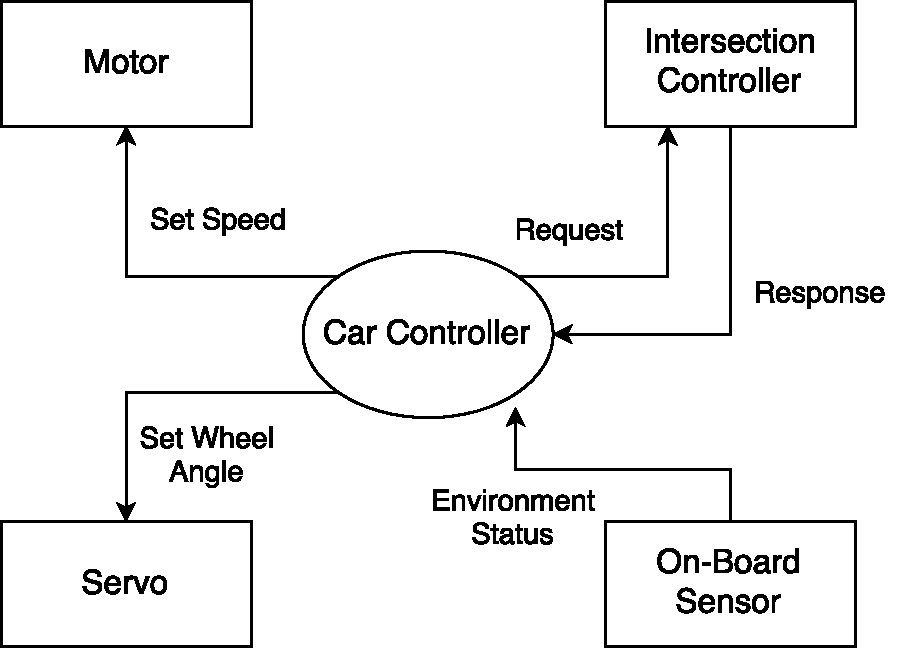
\includegraphics [scale =0.8] {figures/CarCtrl_ContextDiag.pdf}

\end{figure}

\break

\begin{figure} [h!]
	\caption{Intersection Controller Context Diagram} \bigskip
	\centering
	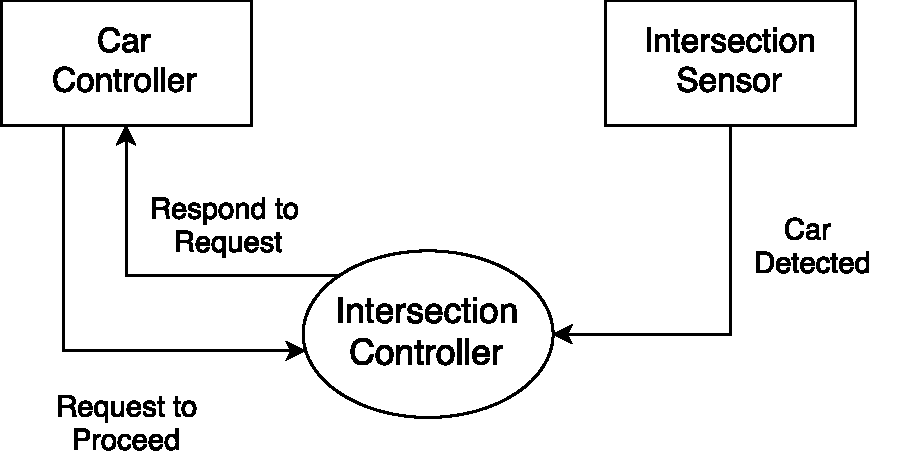
\includegraphics [scale = 0.8] {figures/IC_ContextDiagram.pdf}

\end{figure}

\subsection{System Component Diagrams}
Insert Text or Image Here. 

% -------------- END OVERALL DESIGN DESCRIPTION  ---------------- %




% -------------- START SYSTEM COMPONENTS ---------------- %
\section{System Components}
 
\subsection{Intersection Control Component}


\begin{longtable}{| p{.25\textwidth } | p{.7\textwidth } | }\hline 
\multicolumn{2}{|c|}{\textbf{IDC1}}  \\ \hline 
%

\multicolumn{1}{|c|}{\textbf {\multirow{1}{*}{\centering Description}}} 
					& The Intersection Controller directs traffic at an intersection by communicating with vehicles and determines which order they should proceed\\ \hline

%
\multicolumn{1}{|c|}{\textbf {\multirow{2}{*}{\centering Inputs}}}  
					 & m\_ic\_carSignal[4]  \\\cline{2-2}
                                 &\cellcolor{tableCell}m\_ic\_readSensors[8] \\\hline
%



%
\multicolumn{1}{|c|}{\textbf {\multirow{1}{*}{\centering Outputs}}}  
					 & c\_ic\_carSignal[4]  \\\hline
%

 

\multicolumn{1}{|c|}{\textbf {\multirow{3}{*}{\centering Timing Constraints}}} 
					 & 1 second intersection arrival decision   \\
                                 &\cellcolor{tableCell}1 second intersection schedule  \\
                                 & \multicolumn{1}{l |}{0.5 second intersection departure decision} \\ \hline

\multicolumn{1}{|c|}{\textbf {\multirow{1}{*}{\centering Deadline}}} 
					 & Decisions must be made before the next intersection arrival poll  \\ \hline



\multicolumn{1}{|c|}{\textbf {\multirow{2}{*}{\centering Initialization}}} & \cellcolor{tableCell}Connect to autonomous vehicles over Bluetooth communication  \\
                                 &Clear all intersection arrival queues \\ \hline
\end{longtable}

% Vehicle Component 
\subsection{Vehicle Controller Component}
\begin{longtable}{| p{.25\textwidth } | p{.7\textwidth } | }\hline 
\multicolumn{2}{|c|}{\textbf{VCD1}}  \\ \hline 
%

\multicolumn{1}{|c|}{\textbf {\multirow{3}{*}{\centering Description}}} & A 1:10 scale RC car will be controlled by the Vehicle Controller. The vehicle will be able to follow lanes and stop at intersections. It will communicate with an Intersection Controller and proceed through the intersection after receiving the appropriate signal from it\\ \hline 

%
\multicolumn{1}{|c|}{\textbf {\multirow{4}{*}{\centering Inputs}}}  & m\_vc\_videoCapture[x][y]  \\\cline{2-2}
                                 &\cellcolor{tableCell}m\_vc\_frontDistance \\
                                 & \multicolumn{1}{l |}{m\_vc\_hallEffect} \\ 
                                 & \multicolumn{1}{l |}{\cellcolor{tableCell}m\_ic\_carProceedSignal} \\ \hline
%
%

%
%
\multicolumn{1}{|c|}{\textbf {\multirow{4}{*}{\centering Outputs}}}  & c\_vc\_ wheelAngle \\
                                 &\cellcolor{tableCell}c\_vc\_carSpeed \\
                                 & \multicolumn{1}{l |}{c\_vc\_vehicleBreak} \\ 
                                 &\cellcolor{tableCell}c\_vc\_requestTheIC \\\hline 
%
%



\multicolumn{1}{|c|}{\textbf {\multirow{1}{*}{\centering Timing Constraints}}} 
					 & Process images within 20 ms  \\ \hline

\multicolumn{1}{|c|}{\textbf {\multirow{3}{*}{\centering Initialization}}} 
					 & \cellcolor{tableCell}Initialize all speed controls to zero  \\
                                 &Initialize wheel angle to zero\\
                                 & \multicolumn{1}{l |}{\cellcolor{tableCell}Connect to intersection over Bluetooth communication} \\ \hline
\end{longtable}

% -------------- END SYSTEM COMPONENTS  ---------------- %


\section{Module Guide}


% IC modules - hardware and software
\subsection{Intersection Controller Modules}

\begin{longtable}{ |p{0.1\textwidth }  | p{0.2\textwidth } |  p{0.3\textwidth } |  p{0.3\textwidth } |}  \hline
    
    \textbf{ID} & \textbf{Name} &  \textbf{Responsibilities} & \textbf{Secrets} \\ \hline
    
    \cellcolor{tableCell}ICM.1  & \cellcolor{tableCell}DecisionMaker & \cellcolor{tableCell}Determine order of car progression & \cellcolor{tableCell} Scheduling algorithm \\ \hline
    
    ICM.2 & VehicleDetection & Know when a car is on top of one of the intersection sensors, and the corresponding sensor & Relationship between magnetic sensor and car \\ \hline
    
    \cellcolor{tableCell}ICM.3  & \cellcolor{tableCell}Communication & \cellcolor{tableCell}Interpret receiving car signals and sending signals to a car & \cellcolor{tableCell}Communication protocol \\ \hline
    
    
        ICM.4 & IC\_Main & Control information flow of intersection controller & Manages intersection modules \\ \hline

\end{longtable}






%  Vehicle Hardware modules
\subsection{Vehicle Controller Hardware Modules}

\begin{longtable}{ |p{0.1\textwidth }  | p{0.2\textwidth } |  p{0.3\textwidth } |  p{0.3\textwidth } |}  \hline
    
    \textbf{ID} & \textbf{Name} &  \textbf{Responsibilities} & \textbf{Secrets} \\ \hline 
    
    
    \cellcolor{tableCell}VCM.1  & \cellcolor{tableCell}SignalConverter & \cellcolor{tableCell}Convert a software signals to a physical signal, and vice versa & \cellcolor{tableCell}How to convert signal  \\ \hline
    
    VCM.2 & SpeedConverter & Convert wheel rotation count to a speed value & Speed calculation algorithm \\ \hline
    
    \cellcolor{tableCell}VCM.3  & \cellcolor{tableCell}ServoController & \cellcolor{tableCell}Set a physical wheel angle & 
    \cellcolor{tableCell}How to convert a software value to a PWM (Pulse Width Modulation) signal \\ \hline
    
    VCM.4 & MotorSpeedController & Control PWM signal & How to convert speed into a PWM signal \\ \hline\hline
    
    \cellcolor{tableCell}VCM.5  & \cellcolor{tableCell}MotorHBridge \newline Controller & \cellcolor{tableCell}Setting H bridge gates & \cellcolor{tableCell}Which gates correspond to which action of the motor  \\ \hline
    
    
\end{longtable}


%  Vehicle Software modules
\subsection{Vehicle Controller Software Modules}

\begin{longtable}{ |p{0.1\textwidth }  | p{0.2\textwidth } |  p{0.3\textwidth } |  p{0.3\textwidth } |}  \hline
    
    \textbf{ID} & \textbf{Name} &  \textbf{Responsibilities} & \textbf{Secrets} \\ \hline
    
    \cellcolor{tableCell}VCM.6  &\cellcolor{tableCell}ImageProcessing &\cellcolor{tableCell}Interpret image into environment state &\cellcolor{tableCell}Image processing algorithm  \\ \hline
    
    VCM.7 & VehicleNavigaton & Control the navigation of the car & How the car navigates on the track \\ \hline
    % \cellcolor{tableCell}VCM.7.1 & \cellcolor{tableCell}VehicleNavigaton\_\newline Speed  & \cellcolor{tableCell}Ensure car speed is maintained at desired speed range & \cellcolor{tableCell}Speed control algorithm \\ \hline
    % VCM.7.2 & VehicleNavigaton\_\newline LanePositioning  & Car position with respect to lane & How to stay in lane \\ \hline
    
    \cellcolor{tableCell}VCM.8  & \cellcolor{tableCell}Communication & \cellcolor{tableCell}Interpret signal from Intersection Controller. Prepare and send signal to the Intersection Controller & \cellcolor{tableCell}Communication Protocol \\ \hline

    VCM.9 & VC\_Main & Control information flow of the car & Manage car modules \\ \hline
    
\end{longtable}



% % -------------- START SUBSYSTEM COMPONENTS ---------------- %
% \section{Subsystem Components}

% \subsection{Hardware}

% \subsubsection{The First Hardware Component}
% \begin{longtable}{| p{.25\textwidth } | p{.7\textwidth } | }\hline 
% \textbf{Identification} & - \\ \hline
% \textbf{Inputs} & - \\ \hline
% \textbf{Outputs} & - \\ \hline
% \textbf{Description} & Insert Description Here\\ \hline 
% \textbf{Timing Constraints} & Insert Timing Constraints Here\\ \hline 
% \textbf{Initialization} & Insert Initialization Stuff Here\\ \hline 
% \end{longtable}

% \subsubsection{The Second Hardware Component}
% \begin{longtable}{| p{.25\textwidth } | p{.7\textwidth } | }\hline 
% \textbf{Identification} & - \\ \hline
% \textbf{Inputs} & - \\ \hline
% \textbf{Outputs} & - \\ \hline
% \textbf{Description} & Insert Description Here\\ \hline 
% \textbf{Timing Constraints} & Insert Timing Constraints Here\\ \hline 
% \textbf{Initialization} & Insert Initialization Stuff Here\\ \hline 
% \end{longtable}

% \subsection{Software}
% \subsubsection{The First Software Component (MIS)}
% \begin{longtable}{| p{.25\textwidth } | p{.7\textwidth } | }\hline 
% \textbf{Identification} & - \\ \hline
% \textbf{Inputs} & - \\ \hline
% \textbf{Outputs} & - \\ \hline
% \textbf{Description} & Insert Description Here\\ \hline 
% \textbf{Timing Constraints} & Insert Timing Constraints Here\\ \hline 
% \textbf{Initialization} & Insert Initialization Stuff Here\\ \hline 
% \end{longtable}

% \subsubsection{The Second Software Component (MIS)}
% \begin{longtable}{| p{.25\textwidth } | p{.7\textwidth } | }\hline 
% \textbf{Identification} & - \\ \hline
% \textbf{Inputs} & - \\ \hline
% \textbf{Outputs} & - \\ \hline
% \textbf{Description} & Insert Description Here\\ \hline 
% \textbf{Timing Constraints} & Insert Timing Constraints Here\\ \hline 
% \textbf{Initialization} & Insert Initialization Stuff Here\\ \hline 
% \end{longtable}


% % -------------- END SUBSYSTEM COMPONENTS  ---------------- %


% -------------- START MIS---------------- %
\section{Module Interface Specification}




\begin{longtable}{| p{.35\textwidth } | p{.6\textwidth } | }\caption{ICM.1 DecisionMaker} \\\hline  
 \multicolumn{2}{|l|}{\textbf {ICM.1 DecisionMaker}}\\ \hline
 
\cellcolor{tableCell}DecisionMaker()& \cellcolor{tableCell}Constructor to initialize the scheduling algorithm \\ \hline 

getSchedule(cars[ ]) : carQueue & When function is called, it will return a queue of cars in the order which they should proceed. Expects an array of car objects when called\\ \hline 

%\cellcolor{tableCell}Constructor/Method 3 & \cellcolor{tableCell}- Description \newline - Description  
%\\ \hline


%Constructor/Method 2 & - Description 4 \newline - Description 4  \\ \hline
\end{longtable}

\begin{longtable}{| p{.35\textwidth } | p{.6\textwidth } | }\caption{ICM.2 VehicleDetection} \\\hline  
 \multicolumn{2}{|l|}{\textbf {ICM.2 VehicleDetection}}\\ \hline
 
\cellcolor{tableCell}VehicleDet()& \cellcolor{tableCell}Constructor to initialize the detection of vehicles at the intersection. \\ \hline 

getSignalsState( ) : bool[ ] & Returns the state of the sensors at the intersection when the function is called. Returns an array of boolean values signifying if the sensors have been tripped or not. \\ \hline 

%\cellcolor{tableCell}Constructor/Method 3 & \cellcolor{tableCell}- Description \newline - Description  
%\\ \hline


%Constructor/Method 2 & - Description 4 \newline - Description 4  \\ \hline
\end{longtable}

\begin{longtable}{| p{.35\textwidth } | p{.6\textwidth } | }\caption{ICM.3 Communication} \\\hline  
 \multicolumn{2}{|l|}{\textbf {ICM.3 Communication}}\\ \hline
 
\cellcolor{tableCell}RecieveRequest() : Request& \cellcolor{tableCell}Function to allow the controller recieve a request to be scheduled from the car.\\ \hline 


\cellcolor{tableCell}SendResponse(car c) : void & \cellcolor{tableCell}Function that allows the intersectrion to send a car the response to proceed through the intersection. \\ \hline




%Constructor/Method 2 & - Description 4 \newline - Description 4  \\ \hline
\end{longtable}

\begin{longtable}{| p{.35\textwidth } | p{.6\textwidth } | }\caption{ICM.4 IC\_Main} \\\hline  
 \multicolumn{2}{|l|}{\textbf {ICM.4 IC\_Main}}\\ \hline
 
\cellcolor{tableCell}Main( ) & \cellcolor{tableCell}Main Function for VIC. \\ \hline 


%\cellcolor{tableCell}Constructor/Method 3 & \cellcolor{tableCell}- Description \newline - Description  
%\\ \hline


%Constructor/Method 2 & - Description 4 \newline - Description 4  \\ \hline
\end{longtable}


\begin{longtable}{| p{.35\textwidth } | p{.6\textwidth } | }\caption{VCM.6 ImageProcessing} \\\hline  
 \multicolumn{2}{|l|}{\textbf {VCM.6 ImageProcessing}}\\ \hline
\cellcolor{tableCell}ImgProc( ) & \cellcolor{tableCell}Function to capture images of the track environment from a webcam and process it into information that can be analysed by software.  \\ \hline 

getImageInfo( ) : ADT & Function to relay image information when called.  \\ \hline 


\end{longtable}

\begin{longtable}{| p{.35\textwidth } | p{.6\textwidth } | }\caption{VCM.7 VehicleNavigation} \\\hline  
 \multicolumn{2}{|l|}{\textbf {VCM.7 VehicleNavigation}}\\ \hline
\cellcolor{tableCell}VehicleNav( ) & \cellcolor{tableCell}Function to signal to the vehicle if there is a change in the navigation, and if so, what changes should be made. \\ \hline 

GetCarState( ) : enum &Function to relay the car state. Will return the states as an enum. Exact states will be determined later. \\ \hline 

\cellcolor{tableCell}driveThroughIntersection( ) : void & \cellcolor{tableCell}Function to signal the car to proceed through the intersection. 
\\ \hline

\end{longtable}

\begin{longtable}{| p{.35\textwidth } | p{.6\textwidth } | }\caption{VCM.8 Communication} \\\hline  
 \multicolumn{2}{|l|}{\textbf {VCM.8 Communication}}\\ \hline
\cellcolor{tableCell}SendRequest(Request r) : void & \cellcolor{tableCell}Function to allow the car to send a request to the interection controller. \\ \hline 

Recieve Response( ) : Car &Function to allow the vehicle to revice a response to proceed from the intersection controller. \\ \hline 

\end{longtable}

\begin{longtable}{| p{.35\textwidth } | p{.6\textwidth } | }\caption{VCM.9 VC\_Main} \\\hline  
 \multicolumn{2}{|l|}{\textbf {VCM.9 VC\_Main}}\\ \hline
\cellcolor{tableCell}VC\_Main& \cellcolor{tableCell}Function to control all software aspects of the vehicle control.  \\ \hline 

\end{longtable}
% -------------- END MIS---------------- 







% % -------------- START MID---------------- %
% \section{Module Interface Design}
% \subsection {MID 1}



% \begin{longtable}{| p{.2\textwidth } | p{.75\textwidth } | }\hline 
% \textbf{Insert Text Here} & \textbf{Insert Text Here} \\ \hline
% \textbf{Insert Text Here} & -\\ \hline 
% \end{longtable}


% \subsection {MID 2 }

% \begin{longtable}{| p{.2\textwidth } | p{.75\textwidth } | }\hline 
% \textbf{Insert Text Here} & \textbf{Insert Text Here} \\ \hline
% \textbf{Insert Text Here} & -\\ \hline 
% \end{longtable}


% \subsection {MID ETC}

% \begin{longtable}{| p{.2\textwidth } | p{.75\textwidth } | }\hline 
% \textbf{Insert Text Here} & \textbf{Insert Text Here} \\ \hline
% \textbf{Insert Text Here} & -\\ \hline 
% \end{longtable}

% -------------- END MID ---------------- %

%% -------------- START FUNCTION TABLES---------------- %
%\section{Function Tables}
%\subsection {Table 1}
%
%\hl{***NEED TO LOOK UP FUNCTION TABLE STYLES AND IF WE NEED THEM***}
%
%\begin{longtable}{| p{.2\textwidth } | p{.75\textwidth } | }\hline 
%\textbf{Insert Text Here} & \textbf{Insert Text Here} \\ \hline
%\textbf{Insert Text Here} & -\\ \hline 
%\end{longtable}
%
%
%\subsection {Table 2 }
%
%\begin{longtable}{| p{.2\textwidth } | p{.75\textwidth } | }\hline 
%\textbf{Insert Text Here} & \textbf{Insert Text Here} \\ \hline
%\textbf{Insert Text Here} & -\\ \hline 
%\end{longtable}
%
%
%\subsection {Table 3}
%
%\begin{longtable}{| p{.2\textwidth } | p{.75\textwidth } | }\hline 
%\textbf{Insert Text Here} & \textbf{Insert Text Here} \\ \hline
%\textbf{Insert Text Here} & -\\ \hline 
%\end{longtable}
%
%% -------------- END FUNCTION TABLES ---------------- %


% -------------- START REFERENCES ---------------- %
\section{References}
\textbf{Possible References Here}

% -------------- END REFERENCES ---------------- %

\end{document}
